% Provenance (never printed): old premiere S material on magmatic rocks (volcanic
% and plutonic textures and cooling rate; basalt/gabbro, andesite/diorite,
% rhyolite/granite; order of crystallisation, told). Cooling of sheets from
% figdata/grade-11/dyke_cooling.py (Delaney 1986 parameters; kappa from England
% et al. 2007). Fractional crystallisation is Year 2's; metamorphism (contact
% aureoles) is g12.03's: not developed here.
\chapter{Igneous Rocks}\label{ch:g11:igneous-rocks}

On the north coast of Ireland, stone columns packed side by side step down
into the sea: the Giant's Causeway, a basalt that
cooled from a lava. In Yosemite, in California, the granite wall of El
Capitan rises some \qty{900}{m} above the valley floor, a single body of
coarse-grained rock. Both crystallised from magma. The basalt cooled at the
surface, its crystals too small to see; the granite cooled deep below ground,
its crystals large enough to see, and it is visible today only because
the rocks above it have been worn away. This chapter reads in a rock's grains
how fast, and how deep, it cooled.
% ledger: photo:g11-giants-causeway, photo:g11-el-capitan, tulane:intrusions

\begin{omfigure}
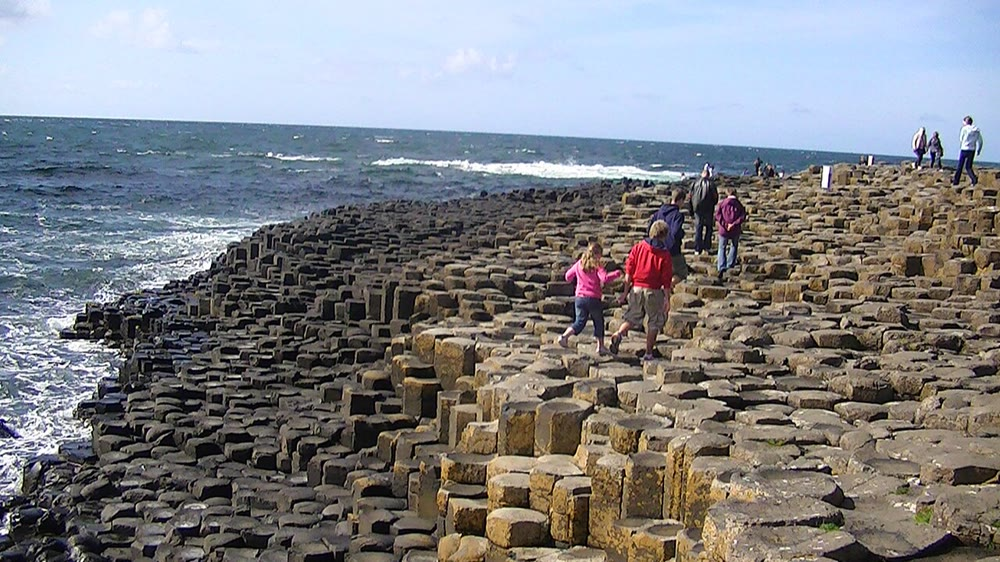
\includegraphics[height=4.3cm]{images/book2/g11-bishop-giants-causeway.jpg}\hspace{0.04\linewidth}%
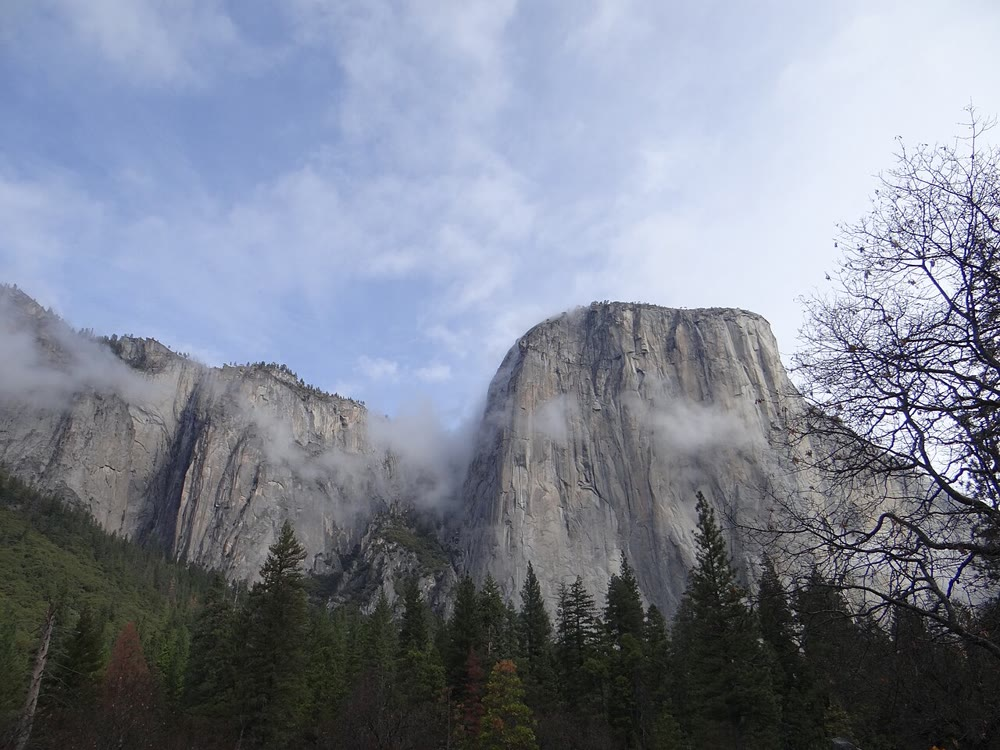
\includegraphics[height=4.3cm]{images/book2/g11-usgs-el-capitan.jpg}

{\small Left: basalt columns of the Giant's Causeway, Northern Ireland.
Photograph Adam Bishop (CC~BY-SA~3.0). Right: El Capitan, Yosemite,
California, a wall of granite about \qty{900}{m} high. Photograph U.S.
Geological Survey (CC0).}
\end{omfigure}
% ledger: photo:g11-giants-causeway, photo:g11-el-capitan

\begin{recall}
Magma is molten rock beneath the surface; it erupts as lava, gently or
explosively (Book 1, grade 7). An igneous rock is one formed when molten
rock cools and becomes solid (Book 1, grade 6). Basalt is a dark \omterm{def:g11:igneous-rocks:volcanic-plutonic}{volcanic rock}, granite a
light rock made of feldspar, quartz and mica (Book 1, grade 6). Mantle
\omterm{def:g11:ocean-ridges:peridotite}{peridotite} melts partly as it rises beneath a ridge, giving the basalt and
\omterm{def:g11:ocean-ridges:gabbro}{gabbro} of the \omterm{def:g11:ocean-ridges:oceanic-lithosphere}{oceanic crust} (\cref{ch:g11:ocean-ridges}). The \omterm{def:g11:minerals:rock-forming}{rock-forming
silicates} are olivine, pyroxenes, amphiboles, micas, feldspars and quartz;
the feldspars are potassium feldspar and plagioclase, a series from
calcium-rich to sodium-rich (\cref{ch:g11:minerals}). Heat spreads by
conduction over a distance of about $\sqrt{\kappa t}$ in a time $t$, where
$\kappa$ is the thermal diffusivity (\cref{ch:g11:subduction-zones}).
\end{recall}
% ledger: tulane:ridge-rocks, england:kelvin

\section{Volcanic and plutonic rocks}

\begin{definition}[Volcanic rock; plutonic rock]\label{def:g11:igneous-rocks:volcanic-plutonic}
An igneous rock, formed by the crystallisation of a magma, is
\emph{volcanic}\index{volcanic rock}
(or extrusive) when the magma solidified at the Earth's surface, as a lava,
and \emph{plutonic}\index{plutonic rock} (or intrusive) when it crystallised
at depth, inside other rocks.
\end{definition}
% ledger: tulane:magma-types

The difference shows in the size of the crystals. A crystal grows by adding
atoms taken from the liquid around it, and that takes time. At the surface,
a lava loses its heat to the air or water fast: material erupted into air or
water cools in seconds, a lava flow in days to weeks. Deep down the
surrounding rocks are hot and the magma loses its heat slowly: a shallow
\omterm{def:g11:igneous-rocks:intrusion}{intrusion} cools in months to years, a large deep one may take millions of
years. Fast cooling gives many small crystals, or none at all; slow cooling
gives fewer, much larger ones.
% ledger: tulane:cooling-times, tulane:textures

\begin{definition}[Texture]\label{def:g11:igneous-rocks:texture}
The \emph{texture}\index{texture (of a rock)} of a rock is the size, shape
and arrangement of its grains. An igneous rock is \emph{glassy} when it
has no crystals, \emph{fine-grained} when its crystals are too small to be
told apart with the naked eye, and \emph{coarse-grained} when they can all
be seen.
\end{definition}
% ledger: tulane:textures

A lava quenched before any crystal can grow becomes a glass: obsidian, black
and glassy, breaks with the conchoidal fracture of a bottle. Basalt is
fine-grained: in the hand its minerals cannot be identified, and even in
\omterm{def:g11:minerals:thin-section}{thin section} the crystals are small (the basalt of \cref{ch:g11:minerals}).
Granite, \omterm{def:g11:ocean-ridges:gabbro}{gabbro} and \omterm{def:g11:igneous-rocks:rock-names}{diorite} are coarse-grained: every grain shows.
% ledger: photo:g11-obsidian, photo:g11-basalt, tulane:textures

\begin{definition}[Phenocryst; porphyritic]\label{def:g11:igneous-rocks:porphyritic}
A \emph{phenocryst}\index{phenocryst} is a large crystal set in a mass of
much smaller crystals or glass, the \emph{groundmass}. A rock with
phenocrysts is \emph{porphyritic}\index{porphyritic}.
\end{definition}
% ledger: tulane:textures

A \omterm{def:g11:igneous-rocks:porphyritic}{porphyritic} \omterm{def:g11:igneous-rocks:texture}{texture} records two stages of cooling: first slow, at depth,
while the \omterm{def:g11:igneous-rocks:porphyritic}{phenocrysts} grew in a magma that was still mostly liquid; then
fast, when the magma rose and erupted, or was injected into cold rock, and
the rest of the liquid froze into the groundmass.
% ledger: tulane:textures

\begin{omfigure}
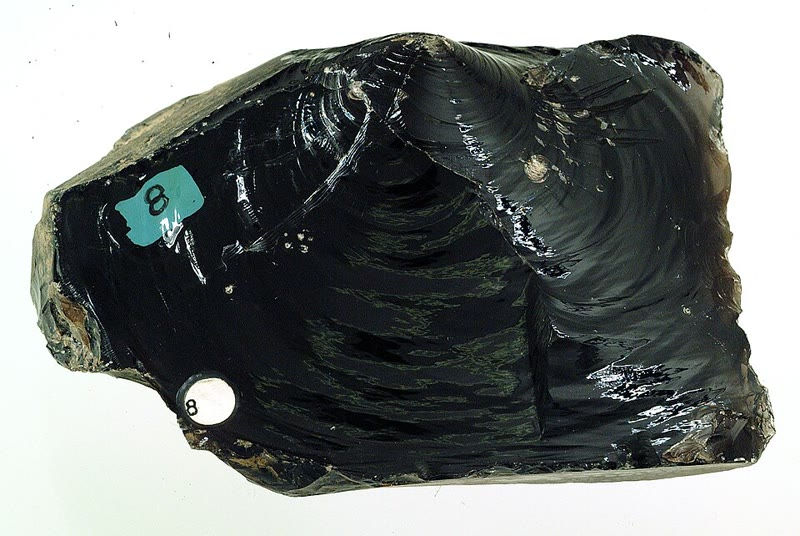
\includegraphics[height=2.75cm]{images/book2/g11-geodil-obsidian.jpg}\hfill
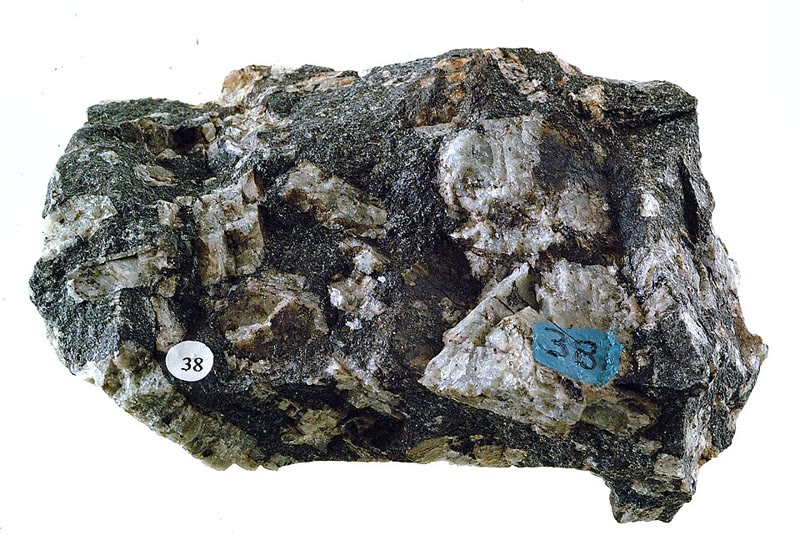
\includegraphics[height=2.75cm]{images/book2/g11-geodil-diabase-porphyry.jpg}\hfill
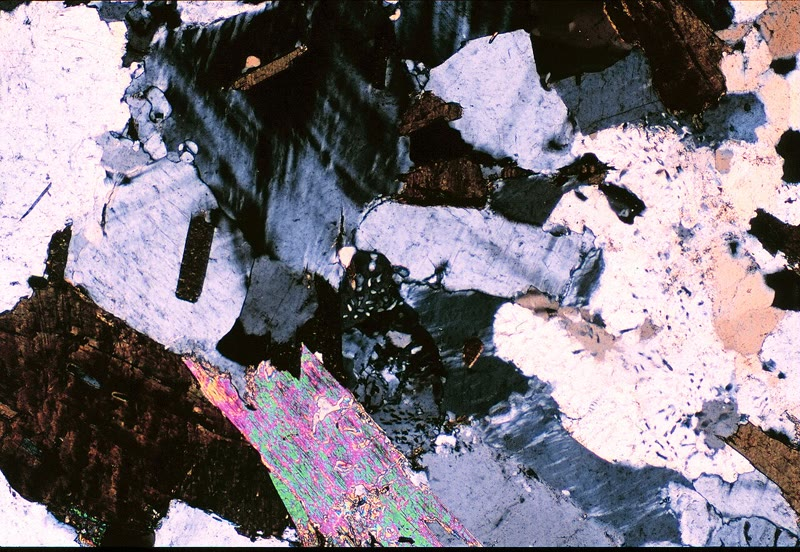
\includegraphics[height=2.75cm]{images/book2/g11-geodil-granite-xpl.jpg}\hfill
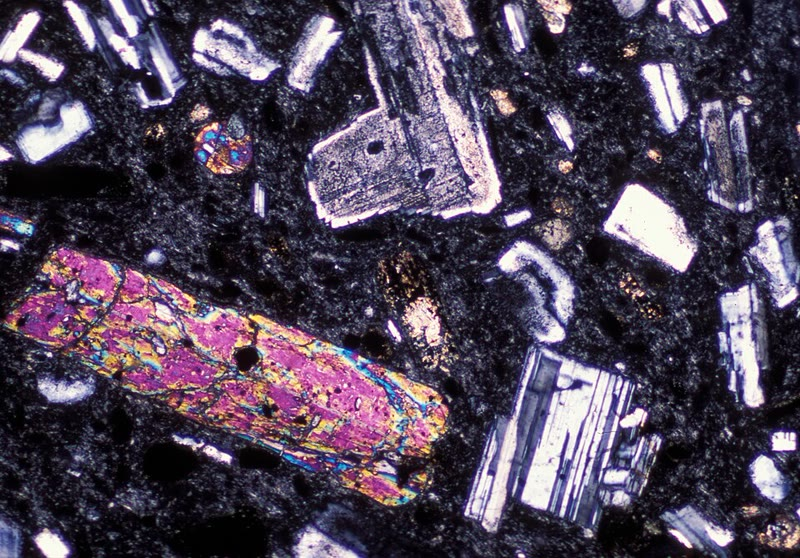
\includegraphics[height=2.75cm]{images/book2/g11-geodil-andesite-xpl.jpg}

{\small From left to right: obsidian, a \omterm{def:g11:igneous-rocks:volcanic-plutonic}{volcanic} glass, with its curved
conchoidal fracture (\qty{9.5}{cm} across); a \omterm{def:g11:igneous-rocks:porphyritic}{porphyritic} rock, blocky
plagioclase \omterm{def:g11:igneous-rocks:porphyritic}{phenocrysts} in a finer groundmass (\qty{9}{cm}); then two
\omterm{def:g11:minerals:thin-section}{thin sections} between crossed polars: a granite, all grains large and
interlocked --- brown biotite, a brightly coloured muscovite, striped
plagioclase, grey and white quartz; an \omterm{def:g11:igneous-rocks:rock-names}{andesite}, \omterm{def:g11:igneous-rocks:porphyritic}{phenocrysts} of
plagioclase and amphibole in a fine-grained groundmass. Photographs Twyla
Baker, Mike Davis and Darla Sondrol, Geology Digital Image Library (CC0).}
\end{omfigure}
% ledger: photo:g11-obsidian, photo:g11-diabase-porphyry, photo:g11-granite-xpl, photo:g11-andesite-xpl

\section{Naming igneous rocks}

The second key to an igneous rock is its chemistry, and above all its
content of silica, \ce{SiO2}, which ranges in common magmas from about
\qty{45}{\percent} to about \qty{75}{\percent} of the mass.

\begin{definition}[Mafic; intermediate; felsic]\label{def:g11:igneous-rocks:felsic-mafic}
A magma, or the rock it forms, is \emph{mafic}\index{mafic} when it holds
about \qty{45}{\percent} to \qty{55}{\percent} \ce{SiO2} and is rich in
iron, magnesium and calcium; \emph{intermediate}\index{intermediate (rock)}
between \qty{55}{\percent} and \qty{65}{\percent}; \emph{felsic}\index{felsic}
when it holds about \qty{65}{\percent} to \qty{75}{\percent} \ce{SiO2} and is
poor in iron, magnesium and calcium but rich in sodium and potassium.
\end{definition}
% ledger: tulane:magma-types, earle:magma-oxides

Each kind of magma gives two rocks, one \omterm{def:g11:igneous-rocks:volcanic-plutonic}{volcanic} and fine-grained, one
\omterm{def:g11:igneous-rocks:volcanic-plutonic}{plutonic} and coarse-grained, with the same chemistry. Basalt and \omterm{def:g11:ocean-ridges:gabbro}{gabbro} are
the \omterm{def:g11:igneous-rocks:felsic-mafic}{mafic} pair, met with the \omterm{def:g11:ocean-ridges:oceanic-lithosphere}{oceanic crust}; granite is the \omterm{def:g11:igneous-rocks:felsic-mafic}{felsic} \omterm{def:g11:igneous-rocks:volcanic-plutonic}{plutonic
rock}. Three names complete the set.

\begin{definition}[Andesite; diorite; rhyolite]\label{def:g11:igneous-rocks:rock-names}
\emph{Andesite}\index{andesite} and \emph{diorite}\index{diorite} are the
\omterm{def:g11:igneous-rocks:volcanic-plutonic}{volcanic} and the \omterm{def:g11:igneous-rocks:volcanic-plutonic}{plutonic rock} of \omterm{def:g11:igneous-rocks:felsic-mafic}{intermediate} composition, made mostly of
plagioclase with amphibole or pyroxene. \emph{Rhyolite}\index{rhyolite} is
the \omterm{def:g11:igneous-rocks:volcanic-plutonic}{volcanic rock} of \omterm{def:g11:igneous-rocks:felsic-mafic}{felsic} composition, the fine-grained equivalent of
granite.
\end{definition}
% ledger: tulane:magma-types, earle:bowen, photo:g11-andesite, photo:g11-diorite

\begin{omfigure}
\begin{tikzpicture}[font=\footnotesize, x=0.4cm]
  % columns: SiO2 45 to 75 % mapped to x = 45 to 75 (0.4 cm per %)
  \begin{scope}[xshift=-18cm]
  \fill[omLithBasalt!45] (45,0) rectangle (55,2.4);
  \fill[omLithBasalt!20] (55,0) rectangle (65,2.4);
  \fill[omLithGranite!45] (65,0) rectangle (75,2.4);
  \draw[black!60] (45,0) rectangle (75,2.4);
  \draw[black!60] (55,0) -- (55,2.4); \draw[black!60] (65,0) -- (65,2.4);
  \draw[black!60] (45,1.2) -- (75,1.2);
  \foreach \x/\a/\b in {50/basalt/gabbro, 60/andesite/diorite, 70/rhyolite/granite}{
    \node[font=\small\bfseries, text height=1.6ex, text depth=0.3ex] at (\x,1.8) {\a};
    \node[font=\small\bfseries, text height=1.6ex, text depth=0.3ex] at (\x,0.6) {\b};}
  \node[anchor=east, align=right] at (44.4,1.8) {fine-grained\\(volcanic)};
  \node[anchor=east, align=right] at (44.4,0.6) {coarse-grained\\(plutonic)};
  \node[anchor=south] at (50,2.45) {mafic};
  \node[anchor=south] at (60,2.45) {intermediate};
  \node[anchor=south] at (70,2.45) {felsic};
  % minerals (a drawing: where each mineral is common)
  \foreach \y/\a/\b/\m/\c in {-0.55/45.2/52/olivine/omLithBasalt!80!black,
      -1.15/45.2/61/pyroxene/omLithBasalt!65!black,
      -1.75/52/69/amphibole/black!60,
      -2.35/57/74.8/biotite/black!75,
      -2.95/45.2/72/plagioclase/omDef!45,
      -3.55/63/74.8/potassium feldspar/omLithGranite!90!red,
      -4.15/64/74.8/quartz/black!20,
      -4.75/68/74.8/muscovite/black!35}{
    \fill[\c] (\a,\y) .. controls ({\a+1.2},{\y+0.22}) and ({\b-1.2},{\y+0.22}) .. (\b,\y)
              .. controls ({\b-1.2},{\y-0.22}) and ({\a+1.2},{\y-0.22}) .. (\a,\y) -- cycle;
    \node[anchor=east] at (44.4,\y) {\m};}
  \node[font=\scriptsize, text=black!75] at (50,-2.95) {calcium-rich};
  \node[font=\scriptsize, text=omDef!80!black, anchor=west] at (72.3,-2.95) {sodium-rich};
  % SiO2 axis
  \draw[-{Stealth[length=4pt]}] (45,-5.35) -- (75.8,-5.35);
  \foreach \x in {45,50,...,75} {\draw (\x,-5.35) -- (\x,-5.45); \node[anchor=north] at (\x,-5.45) {\x};}
  \node[anchor=north] at (60,-5.85) {\ce{SiO2} (\unit{\percent} of the mass)};
  \draw[black!30, dashed] (55,0) -- (55,-5.35); \draw[black!30, dashed] (65,0) -- (65,-5.35);
  \end{scope}
\end{tikzpicture}

{\small Naming the common igneous rocks (a drawing). Columns: the silica
content of the magma; rows: fine-grained (\omterm{def:g11:igneous-rocks:volcanic-plutonic}{volcanic}) and coarse-grained
(\omterm{def:g11:igneous-rocks:volcanic-plutonic}{plutonic}) rocks. Below, where each rock-forming mineral is common: olivine
and pyroxene in \omterm{def:g11:igneous-rocks:felsic-mafic}{mafic} rocks with calcium-rich plagioclase; amphibole and
plagioclase in \omterm{def:g11:igneous-rocks:felsic-mafic}{intermediate} rocks; potassium feldspar, quartz,
sodium-rich plagioclase and micas in \omterm{def:g11:igneous-rocks:felsic-mafic}{felsic} rocks. The boundaries are
gradual.}
\end{omfigure}
% ledger: tulane:magma-types, earle:bowen, earle:magma-oxides, photo:g11-andesite, photo:g11-diorite, photo:g11-granite, nps:granite-minerals

\begin{method}[Naming an igneous rock]\label{met:g11:igneous-rocks:naming}
\begin{enumerate}
  \item Look at the \omterm{def:g11:igneous-rocks:texture}{texture}: glassy, fine-grained or coarse-grained;
        \omterm{def:g11:igneous-rocks:porphyritic}{porphyritic} or not. Fine-grained or glassy means \omterm{def:g11:igneous-rocks:volcanic-plutonic}{volcanic} (or a
        small, quickly cooled \omterm{def:g11:igneous-rocks:intrusion}{intrusion}); coarse-grained means \omterm{def:g11:igneous-rocks:volcanic-plutonic}{plutonic}.
  \item Identify the minerals that can be seen
        (\cref{met:g11:minerals:identify}): quartz and potassium feldspar
        point to \omterm{def:g11:igneous-rocks:felsic-mafic}{felsic}, amphibole with plagioclase to \omterm{def:g11:igneous-rocks:felsic-mafic}{intermediate}, olivine
        and pyroxene to \omterm{def:g11:igneous-rocks:felsic-mafic}{mafic}. In a fine-grained rock, use the \omterm{def:g11:igneous-rocks:porphyritic}{phenocrysts},
        the colour of the groundmass --- dark for \omterm{def:g11:igneous-rocks:felsic-mafic}{mafic}, light for \omterm{def:g11:igneous-rocks:felsic-mafic}{felsic} ---
        as a hint, or a chemical analysis.
  \item Read the name at the crossing of the row and the column of the
        chart.
\end{enumerate}
\end{method}

\begin{example}[Two basalts]
A dark rock from a lava flow is fine-grained throughout; another, from the
same volcano, shows green grains of olivine a few millimetres across in a
dark groundmass. Both are \omterm{def:g11:igneous-rocks:felsic-mafic}{mafic} and fine-grained: both are basalts. The
second is a \omterm{def:g11:igneous-rocks:porphyritic}{porphyritic} basalt: its olivine grew first, slowly, in the
magma below the volcano, before the lava erupted and froze around it.
\end{example}
% ledger: photo:g11-olivine, earle:bowen, tulane:textures

\begin{omfigure}
\makebox[0.32\linewidth]{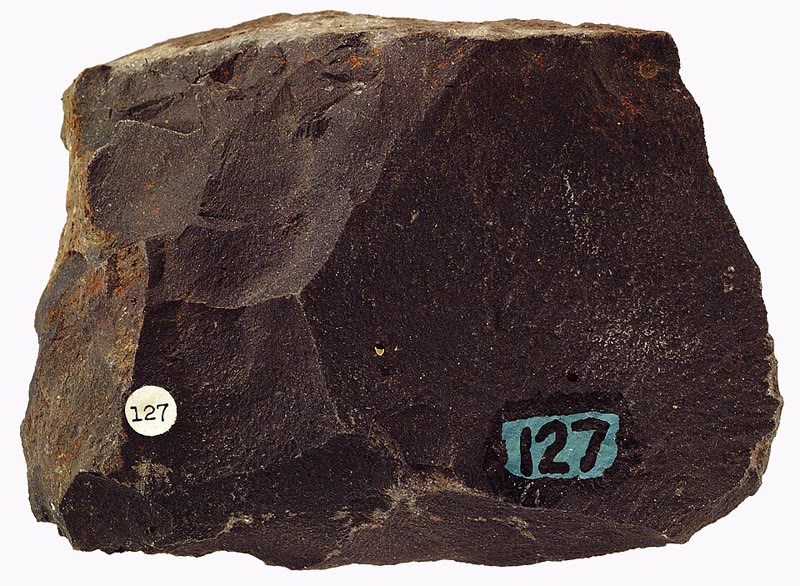
\includegraphics[height=2.9cm]{images/book2/g11-geodil-basalt.jpg}}\hfill
\makebox[0.32\linewidth]{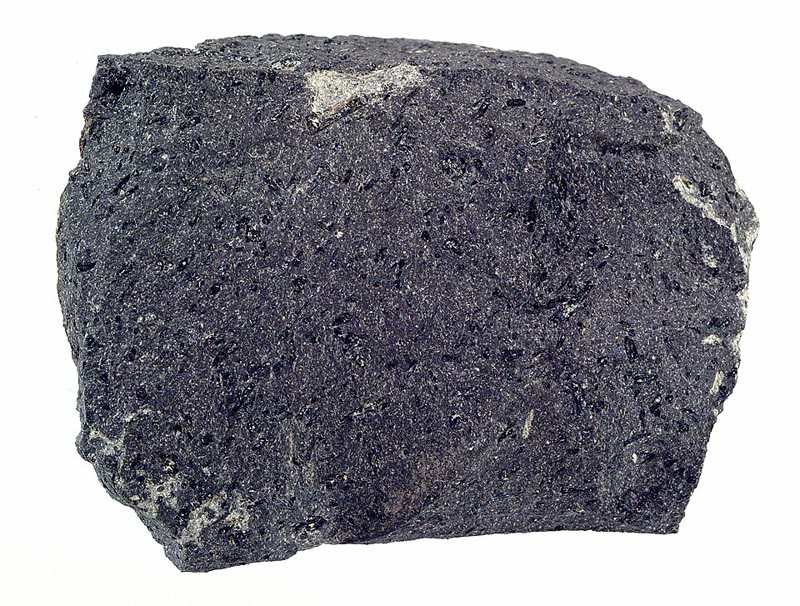
\includegraphics[height=2.9cm]{images/book2/g11-geodil-andesite.jpg}}\hfill
\makebox[0.32\linewidth]{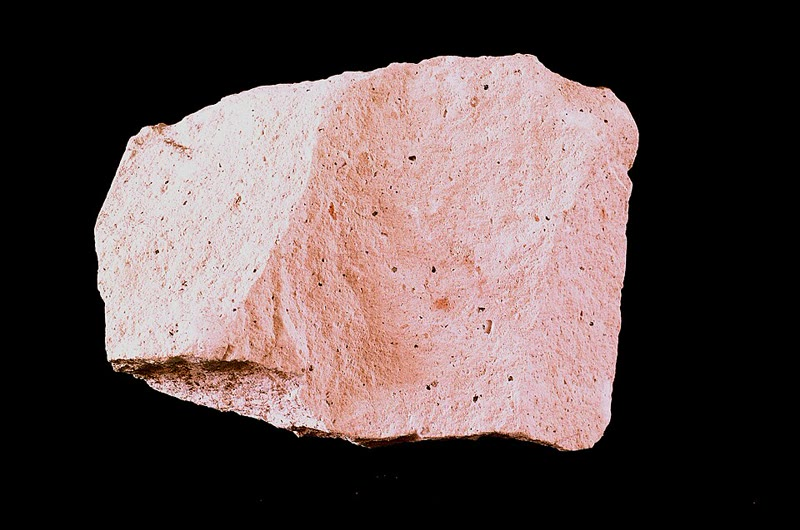
\includegraphics[height=2.9cm]{images/book2/g11-geodil-rhyolite.jpg}}

\smallskip
\makebox[0.32\linewidth]{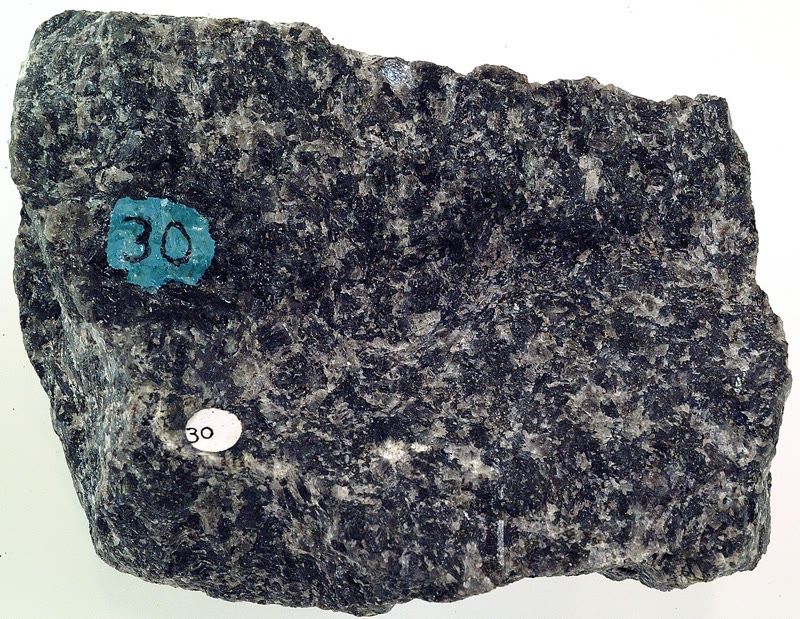
\includegraphics[height=2.9cm]{images/book2/g11-geodil-gabbro.jpg}}\hfill
\makebox[0.32\linewidth]{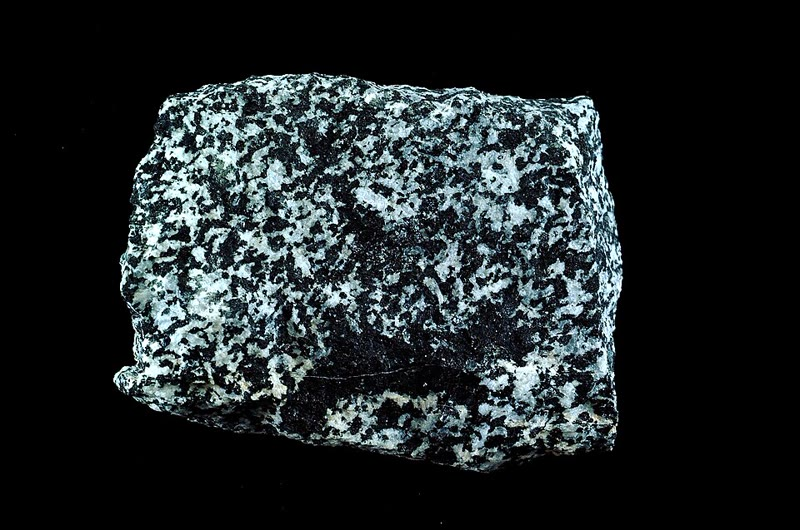
\includegraphics[height=2.9cm]{images/book2/g11-geodil-diorite.jpg}}\hfill
\makebox[0.32\linewidth]{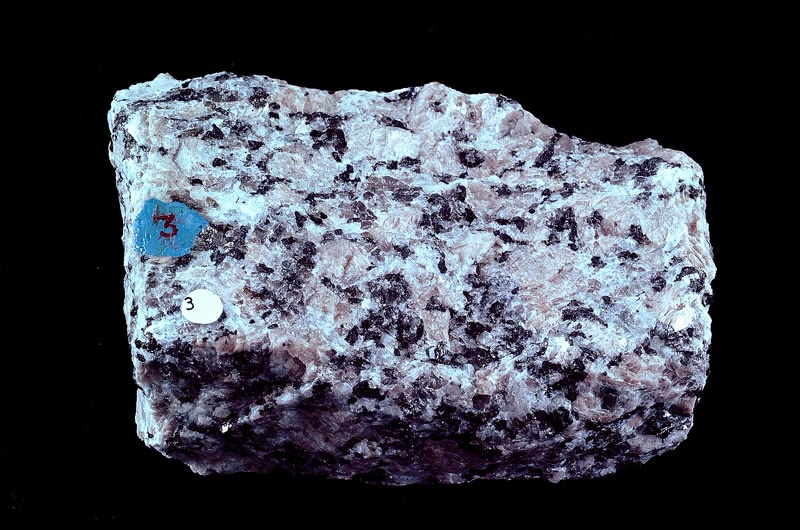
\includegraphics[height=2.9cm]{images/book2/g11-geodil-granite.jpg}}

{\small The three pairs of igneous rocks, \omterm{def:g11:igneous-rocks:felsic-mafic}{mafic} to \omterm{def:g11:igneous-rocks:felsic-mafic}{felsic} from left to right:
\omterm{def:g11:igneous-rocks:volcanic-plutonic}{volcanic} above, \omterm{def:g11:igneous-rocks:volcanic-plutonic}{plutonic} below. Top: a fine-grained basalt; an \omterm{def:g11:igneous-rocks:rock-names}{andesite}, small
amphibole crystals in a fine-grained groundmass (about \qty{10}{cm});
a pink \omterm{def:g11:igneous-rocks:rock-names}{rhyolite}. Bottom: \omterm{def:g11:ocean-ridges:gabbro}{gabbro} (\qty{9}{cm}); \omterm{def:g11:igneous-rocks:rock-names}{diorite}, black hornblende and
glassy plagioclase (\qty{10}{cm}); a coarse granite with large pale pink
potassium feldspars, grey plagioclase, quartz, biotite and hornblende
(\qty{10}{cm}). Photographs Nessa Eull, Twyla Baker, Joseph H.~Hartman,
Darla Sondrol and Dexter Perkins, Geology Digital Image Library (CC0).}
\end{omfigure}
% ledger: photo:g11-basalt, photo:g11-andesite, photo:g11-rhyolite, photo:g11-gabbro, photo:g11-diorite, photo:g11-granite

\section{The order of crystallisation}

A magma does not freeze at one temperature, as water does. Its minerals
appear one after another as it cools, each in its own range of temperature,
so that a cooling magma can hold crystals and still be mostly liquid.

\begin{history}[Bowen's experiments]
Norman L.~Bowen (1887--1956) joined the Geophysical Laboratory of the
Carnegie Institution in Washington in 1912. Working mostly with basaltic
magmas, he melted a rock in a furnace, let it cool slowly to a chosen
temperature so that some minerals formed, then quenched it, cooling it so
fast that the remaining liquid became a glass. Under the microscope, the
crystals showed which minerals had formed above that temperature. Repeated
at lower and lower temperatures, the experiment gave the order in which the
minerals appear. Bowen published this order as a reaction series in 1922
and his book \emph{The Evolution of the Igneous Rocks} in 1928.
\end{history}
% ledger: carnegie:bowen, earle:bowen

\begin{omfigure}
\begin{tikzpicture}[font=\footnotesize, box/.style={draw=black!60, rounded corners=2pt, fill=#1, minimum width=3.0cm, minimum height=0.62cm, align=center}]
  \node[box=omLithBasalt!45] (ol) at (0,0) {olivine};
  \node[box=omLithBasalt!35] (px) at (0,-1.1) {pyroxene};
  \node[box=black!15] (am) at (0,-2.2) {amphibole};
  \node[box=black!25] (bi) at (0,-3.3) {biotite};
  \draw[-{Stealth[length=4pt]}, line width=0.8pt] (ol) -- (px);
  \draw[-{Stealth[length=4pt]}, line width=0.8pt] (px) -- (am);
  \draw[-{Stealth[length=4pt]}, line width=0.8pt] (am) -- (bi);
  \node[align=center, anchor=south] at (0,0.45) {\textbf{discontinuous branch}\\each mineral reacts with the liquid\\into the next};
  % continuous branch: a wedge from Ca-rich to Na-rich
  \fill[left color=omDef!55, right color=omDef!12, shading angle=180] (5.0,-0.9) -- (6.6,-0.9) -- (6.6,-3.5) -- (5.0,-3.5) -- cycle;
  \shade[top color=omDef!60, bottom color=omDef!10, draw=black!60, rounded corners=2pt] (4.3,-0.85) rectangle (7.3,-3.55);
  \node[align=center] at (5.8,-1.3) {calcium-rich\\plagioclase};
  \node[align=center] at (5.8,-3.15) {sodium-rich\\plagioclase};
  \draw[-{Stealth[length=4pt]}, line width=0.8pt] (5.8,-1.65) -- (5.8,-2.7);
  \node[align=center, anchor=south] at (5.8,0.45) {\textbf{continuous branch}\\the plagioclase changes\\gradually};
  % last minerals
  \node[box=omLithGranite!45, minimum width=7.6cm] (last) at (2.9,-4.75) {potassium feldspar, quartz, (muscovite)};
  \draw[-{Stealth[length=4pt]}, line width=0.8pt] (bi) -- (bi |- last.north);
  \draw[-{Stealth[length=4pt]}, line width=0.8pt] (5.8,-3.55) -- (5.8,-4.43);
  % temperature arrow
  \draw[-{Stealth[length=5pt]}, line width=1pt, omThm] (-2.6,0.3) -- (-2.6,-4.9);
  \node[anchor=east, align=right, text=omThm] at (-2.75,0.1) {first,\\\qtyrange{1200}{1300}{\degreeCelsius}};
  \node[anchor=east, align=right, text=omThm] at (-2.75,-4.7) {last, about\\\qtyrange{750}{800}{\degreeCelsius}};
  \node[anchor=east, align=right, text=omThm] at (-2.75,-2.3) {falling\\temperature};
\end{tikzpicture}

{\small The order in which minerals crystallise from a cooling magma
(Bowen's reaction series, a drawing). Olivine forms first; plagioclase starts
at about the point where pyroxene does, rich in calcium at first, then
richer and richer in sodium. Potassium feldspar, quartz and sometimes
muscovite form last, from what remains of a silica-rich liquid.}
\end{omfigure}
% ledger: earle:bowen

The word \emph{reaction} matters. Olivine is stable at high temperature
only: as the magma cools, olivine crystals react with silica in the liquid
and turn into pyroxene,
\[
  \ce{Mg2SiO4 + SiO2 -> 2 MgSiO3},
\]
and so on down the branch, as long as silica remains in the liquid. Along
the other branch, plagioclase crystals keep growing, but each new layer is
richer in sodium than the last: a plagioclase crystal can be zoned, from a
calcium-rich core to a sodium-rich rim, like the plagioclase \omterm{def:g11:igneous-rocks:porphyritic}{phenocrysts} of
the \omterm{def:g11:igneous-rocks:rock-names}{andesite} above.
% ledger: earle:bowen, photo:g11-andesite-xpl

The series explains the chart. A \omterm{def:g11:igneous-rocks:felsic-mafic}{mafic} magma runs out of silica early: it
crystallises olivine, pyroxene and calcium-rich plagioclase, and gives a
\omterm{def:g11:ocean-ridges:gabbro}{gabbro} if it cools slowly underground, a basalt if it cools fast at the
surface. Only a magma rich in silica goes on to the end of the series and
forms potassium feldspar and quartz: the minerals of granite and \omterm{def:g11:igneous-rocks:rock-names}{rhyolite}.
How a magma changes its composition on the way, when its early crystals are
separated from the liquid, is the subject of the second university year.
% ledger: earle:bowen, tulane:bowen

\section{Intrusions}

Magma rises because it is less dense than the rocks around it, forcing its
way into fractures and widening them. Much of it never reaches the surface:
it crystallises in the crust as \omterm{def:g11:igneous-rocks:intrusion}{intrusions}, which are seen only once
erosion has removed the rocks above.
% ledger: tulane:intrusions

\begin{definition}[Dyke; sill; pluton]\label{def:g11:igneous-rocks:intrusion}
An \emph{intrusion}\index{intrusion} is a body of igneous rock that
crystallised inside other rocks. A \emph{dyke}\index{dyke} is a sheet of
igneous rock that cuts across the layers or structures of the rocks it
intrudes; a \emph{sill}\index{sill} is a sheet that lies parallel to the
layers, between them. A \emph{pluton}\index{pluton} is a large intrusion of
any shape, formed at depth; many plutons joined together form a
batholith (\cref{ch:g12:subduction-magmatism}).
\end{definition}
% ledger: tulane:intrusions

\omterm{def:g11:igneous-rocks:intrusion}{Dykes} are commonly less than \qty{20}{m} wide and \omterm{def:g11:igneous-rocks:intrusion}{sills} less than \qty{50}{m}
thick; a \omterm{def:g11:igneous-rocks:intrusion}{sill} is usually fed by a \omterm{def:g11:igneous-rocks:intrusion}{dyke}. Shallow \omterm{def:g11:igneous-rocks:intrusion}{dykes} and \omterm{def:g11:igneous-rocks:intrusion}{sills} cool fast:
they are fine-grained, sometimes \omterm{def:g11:igneous-rocks:porphyritic}{porphyritic}. Against the cold rock they
intrude, their edges cool fastest of all and are even finer grained than
their centre: a \emph{chilled margin}, the mark of a body that was hot when
it came into place. The Sierra Nevada of California, where Yosemite lies,
is a batholith: the granitic rocks whose density was measured in
\cref{ch:g11:minerals} come from about two hundred of its \omterm{def:g11:igneous-rocks:intrusion}{plutons}.
% ledger: tulane:intrusions, usgs91:sierra, photo:g11-el-capitan

\begin{omfigure}
\begin{tikzpicture}[font=\footnotesize, scale=0.9]
  % layered host rocks
  \fill[omLithSand] (0,0) rectangle (14,-1.0);
  \fill[omLithShale] (0,-1.0) rectangle (14,-2.0);
  \fill[omLithLime] (0,-2.0) rectangle (14,-3.0);
  \fill[omLithSand] (0,-3.0) rectangle (14,-4.0);
  \fill[omLithShale] (0,-4.0) rectangle (14,-6.4);
  \foreach \y in {-1,-2,-3,-4} \draw[black!35] (0,\y) -- (14,\y);
  % pluton
  \fill[omLithGranite, draw=black!60] (2.2,-6.4) .. controls (2.4,-4.6) and (3.6,-4.1) .. (5.5,-4.15)
     .. controls (7.4,-4.2) and (9.0,-4.5) .. (9.6,-6.4) -- cycle;
  % sill between the limestone and the shale, fed by the dyke
  \fill[omLithBasalt, draw=black!60] (7.3,-1.88) -- (12.6,-1.88) .. controls (12.9,-1.9) and (12.9,-2.1) .. (12.6,-2.12) -- (7.3,-2.12) -- cycle;
  % dyke from the pluton to the volcano
  \fill[omLithBasalt, draw=black!60] (7.0,-4.18) -- (7.3,-4.2) -- (7.3,0) -- (7.0,0) -- cycle;
  % a second dyke cutting across the layers, not reaching the surface
  \fill[omLithBasalt, draw=black!60] (3.9,-4.15) -- (4.15,-4.15) -- (2.95,-0.6) -- (2.75,-0.6) -- cycle;
  % volcano and lava flow
  \fill[black!65] (5.75,0) -- (7.15,1.35) -- (8.55,0) -- cycle;
  \fill[omLithBasalt!80!black] (8.4,0) -- (11.6,0) -- (11.6,0.1) .. controls (10.5,0.16) and (9.2,0.22) .. (8.3,0.15) -- cycle;
  \draw[black!70] (0,0) -- (5.75,0); \draw[black!70] (8.55,0) -- (14,0);
  % labels
  \node[anchor=south] at (7.15,1.4) {volcano};
  \draw[black!60] (10.5,0.15) -- (11.2,0.8); \node[anchor=south west, inner sep=1pt] at (11.2,0.8) {lava flow};
  \draw[black!60] (7.3,-0.5) -- (8.3,-0.5); \node[anchor=west, fill=omLithSand, inner sep=1pt] at (8.3,-0.5) {dyke (cuts across the layers)};
  \draw[black!60] (11.0,-2.0) -- (11.0,-2.55); \node[anchor=north, fill=omLithLime, inner sep=1pt] at (11.0,-2.55) {sill (between the layers)};
  \draw[black!60] (3.4,-2.5) -- (1.9,-2.5); \node[anchor=east, fill=omLithLime, inner sep=1pt] at (1.9,-2.5) {dyke};
  \node[align=center] at (5.9,-5.5) {pluton};
  \node[anchor=east, fill=omLithShale, inner sep=1pt] at (13.85,-5.3) {layered sedimentary rocks};
\end{tikzpicture}

{\small \omterm{def:g11:igneous-rocks:intrusion}{Intrusions} (a drawing, not to scale). A \omterm{def:g11:igneous-rocks:intrusion}{pluton} crystallises at depth;
\omterm{def:g11:igneous-rocks:intrusion}{dykes} cut across the layers of the rocks above it, one of them feeding a
volcano; a \omterm{def:g11:igneous-rocks:intrusion}{sill} spreads between two layers. Only erosion of the rocks above
lays these bodies bare at the surface.}
\end{omfigure}
% ledger: tulane:intrusions

How long does an \omterm{def:g11:igneous-rocks:intrusion}{intrusion} take to crystallise? Consider a sheet of
magma --- a \omterm{def:g11:igneous-rocks:intrusion}{dyke} or a \omterm{def:g11:igneous-rocks:intrusion}{sill} --- of thickness $b$, losing its heat by
conduction into the rock on both sides. The only quantities that set the
pace are the thickness $b$, in metres, and the thermal diffusivity $\kappa$,
in \unit{m^2/s}; the only time that can be built from them is $b^2/\kappa$.
% ledger: england:kelvin, delaney86:example

\begin{proposition}[The cooling time of a sheet of magma]\label{prop:g11:igneous-rocks:cooling}
A sheet of magma of thickness $b$ that cools by conduction solidifies in a
time
\[
  t = C\,\frac{b^2}{\kappa},
\]
where $\kappa$ is the thermal diffusivity of the rocks and $C$ a number set
by the temperatures of the magma and of the surrounding rock and by the heat
released as the magma crystallises. Doubling the thickness multiplies the
time by four. (Admitted; the value of $C$ comes from a computed model.)
\end{proposition}
% ledger: delaney86:properties, delaney86:example

For a basaltic magma intruded at \qty{1150}{\degreeCelsius} into rock at
\qty{50}{\degreeCelsius}, which crystallises completely at
\qty{950}{\degreeCelsius} and releases \qty{900}{MJ} of heat for each cubic
metre that crystallises, with $\kappa = \qty{1e-6}{m^2/s}$, the model gives
$C \approx 0.21$. A sheet \qty{2}{m} thick then solidifies in about ten
days, a \omterm{def:g11:igneous-rocks:intrusion}{sill} \qty{20}{m} thick in about two and a half years, one
\qty{100}{m} thick in about sixty-five years. Without the heat of
crystallisation, the times would be three times shorter: crystallising
magma keeps itself warm.
% values (dyke_cooling.py): t2_day 9.55, t20_yr 2.61, t100_yr 65.3, latent_factor 2.94; C = 8.2475e7 s / 4e8 s = 0.206
% ledger: delaney86:example, delaney86:properties, england:kelvin

\begin{omfigure}
\begin{tikzpicture}
\begin{axis}[omrecord, name=times, width=0.45\linewidth, height=5.0cm, xmode=log, ymode=log,
  xmin=0.8, xmax=130, ymin=1e-3, ymax=200, xlabel={thickness of the sheet (\unit{m})},
  ylabel={time to solidify (years)},
  legend style={font=\scriptsize, at={(0.5,-0.4)}, anchor=north, legend columns=2,
    /tikz/every even column/.append style={column sep=4pt}}]
% computed in figdata/grade-11/dyke_cooling.py; ledger: delaney86:*, england:kelvin
\addplot[omThm, line width=1pt, mark=*, mark size=1.4pt] table[x=b, y=t_yr] {figdata/out/grade-11-dyke_cooling-times.dat};
\addplot[omDef, line width=1pt, dashed, mark=o, mark size=1.4pt] table[x=b, y=t0_yr] {figdata/out/grade-11-dyke_cooling-times.dat};
\legend{with heat of crystallisation, without}
\end{axis}
\begin{axis}[omrecord, at={(times.east)}, anchor=west, xshift=1.6cm, width=0.45\linewidth, height=5.0cm,
  xmin=-28, xmax=28, ymin=0, ymax=1300, xlabel={distance from the centre of the sill (\unit{m})},
  ylabel={temperature (\unit{\degreeCelsius})},
  legend style={font=\scriptsize, at={(0.5,-0.4)}, anchor=north, legend columns=4,
    /tikz/every even column/.append style={column sep=4pt}}]
\fill[omLithBasalt!30] (axis cs:-10,0) rectangle (axis cs:10,1300);
\draw[black!50, dashed] (axis cs:-28,950) -- (axis cs:28,950);
\node[font=\scriptsize, anchor=south east, text=black!60] at (axis cs:27,955) {solidus};
\node[font=\scriptsize, anchor=north] at (axis cs:0,1290) {sill};
% computed in figdata/grade-11/dyke_cooling.py
\addplot[omProp, line width=0.9pt] table[x=x, y=T1] {figdata/out/grade-11-dyke_cooling-profiles.dat};
\addplot[omThm, line width=0.9pt] table[x=x, y=T2] {figdata/out/grade-11-dyke_cooling-profiles.dat};
\addplot[omDef, line width=0.9pt] table[x=x, y=T3] {figdata/out/grade-11-dyke_cooling-profiles.dat};
\addplot[black, line width=0.9pt] table[x=x, y=T4] {figdata/out/grade-11-dyke_cooling-profiles.dat};
\legend{30 days, 6 months, 1 year, 2 years}
\end{axis}
\end{tikzpicture}

{\small A sheet of basaltic magma cooling by conduction (computed model).
Left: the time it takes to solidify, against its thickness, on logarithmic
axes: a straight line of slope 2, the time growing as the square of the
thickness. Right: temperatures across a \omterm{def:g11:igneous-rocks:intrusion}{sill} \qty{20}{m} thick (shaded),
intruded at \qty{1150}{\degreeCelsius} into rock at
\qty{50}{\degreeCelsius}. The edges fall below the solidus at once, the
centre only after about two and a half years.}
\end{omfigure}
% values (dyke_cooling.py): profiles at 30, 180, 365, 730 days; contact about 690 degC (Delaney: 690)

The model also shows the chilled margin forming. The rock at the contact
jumps at once to about \qty{690}{\degreeCelsius}, far below the solidus: the
first centimetres of the \omterm{def:g11:igneous-rocks:intrusion}{sill} freeze within a day, while its centre stays
liquid for years. Real \omterm{def:g11:igneous-rocks:intrusion}{intrusions} are more complicated --- the properties of
rocks change with temperature, water circulates, a deep \omterm{def:g11:igneous-rocks:intrusion}{pluton} sits in rock
that is already hot and may be fed again and again --- which is why large
deep \omterm{def:g11:igneous-rocks:intrusion}{intrusions} take far longer to cool than the law, with a cold host, would
suggest.
% ledger: delaney86:example, tulane:cooling-times
% values (dyke_cooling.py): margin_day_20m 0.58 (cell 12.5 cm from the contact)

\section{Exercises}

\begin{exercise}[$\star$]\label{exo:g11:igneous-rocks:1}
Define a \omterm{def:g11:igneous-rocks:volcanic-plutonic}{volcanic rock} and a \omterm{def:g11:igneous-rocks:volcanic-plutonic}{plutonic rock}. Give the three pairs of
\omterm{def:g11:igneous-rocks:volcanic-plutonic}{volcanic} and \omterm{def:g11:igneous-rocks:volcanic-plutonic}{plutonic rocks} of the same composition, from \omterm{def:g11:igneous-rocks:felsic-mafic}{mafic} to \omterm{def:g11:igneous-rocks:felsic-mafic}{felsic}.
\end{exercise}

\begin{exercise}[$\star$]\label{exo:g11:igneous-rocks:2}
Match each rock to its \omterm{def:g11:igneous-rocks:texture}{texture} --- glassy, fine-grained, coarse-grained,
\omterm{def:g11:igneous-rocks:porphyritic}{porphyritic}: (1) obsidian; (2) granite; (3) a basalt with green olivine
crystals a few millimetres across in a dark groundmass; (4) a basalt in which
no mineral can be seen.
\end{exercise}

\begin{exercise}[$\star$]\label{exo:g11:igneous-rocks:3}
Three magmas contain \qty{48}{\percent}, \qty{60}{\percent} and
\qty{72}{\percent} \ce{SiO2}. Classify each, and name the rock each gives
when it cools slowly at depth.
\end{exercise}

\begin{exercise}[$\star$]\label{exo:g11:igneous-rocks:4}
Define a \omterm{def:g11:igneous-rocks:intrusion}{dyke}, a \omterm{def:g11:igneous-rocks:intrusion}{sill} and a \omterm{def:g11:igneous-rocks:intrusion}{pluton}. On the drawing of \omterm{def:g11:igneous-rocks:intrusion}{intrusions} in this
chapter, which body fed the volcano?
\end{exercise}

\begin{exercise}[$\star$]\label{exo:g11:igneous-rocks:5}
In Bowen's reaction series, which mineral forms first, and which minerals
form last? How does plagioclase change as the magma cools?
\end{exercise}

\begin{exercise}[$\star\star$]\label{exo:g11:igneous-rocks:6}
Two rocks are analysed (mass percentages). Rock A: \ce{SiO2} 74, \ce{Al2O3}
14, \ce{FeO} 3, \ce{CaO} 3, \ce{MgO} 0.5, \ce{Na2O} 5, \ce{K2O} 4. Rock B:
\ce{SiO2} 47, \ce{Al2O3} 14, \ce{FeO} 8, \ce{CaO} 10, \ce{MgO} 8, \ce{Na2O}
1, \ce{K2O} 2. (1) Classify each. (2) Check your answer with the other
oxides. (3) Rock A is fine-grained: name it. Rock B is coarse-grained: name
it.
\end{exercise}

\begin{exercise}[$\star\star$]\label{exo:g11:igneous-rocks:7}
A \omterm{def:g11:igneous-rocks:intrusion}{dyke} \qty{2}{m} thick solidifies in about ten days. Using the proposition
on the cooling time, how long does a \omterm{def:g11:igneous-rocks:intrusion}{dyke} of the same magma take if it is
\qty{1}{m} thick? A \omterm{def:g11:igneous-rocks:intrusion}{sill} \qty{20}{m} thick? One \qty{200}{m} thick?
\end{exercise}

\begin{exercise}[$\star\star$]\label{exo:g11:igneous-rocks:8}
(1) Show that $b^2/\kappa$ is a time. (2) Compute it for $b = \qty{20}{m}$
and $\kappa = \qty{1e-6}{m^2/s}$, in seconds and in years
($\num{1}\text{ year} \approx \qty{3.16e7}{s}$). (3) With $C = 0.21$, how long
does the \omterm{def:g11:igneous-rocks:intrusion}{sill} take to solidify?
\end{exercise}

\begin{exercise}[$\star\star$]\label{exo:g11:igneous-rocks:9}
A rock shows blocky plagioclase crystals about a centimetre long in a
groundmass whose grains cannot be seen. Describe its \omterm{def:g11:igneous-rocks:texture}{texture}, and tell the
story of its cooling in two stages.
\end{exercise}

\begin{exercise}[$\star\star$]\label{exo:g11:igneous-rocks:10}
Olivine reacts with silica in the liquid: $\ce{Mg2SiO4 + SiO2 -> 2
MgSiO3}$. (1) Check that the equation is balanced. (2) With the molar masses
\qty{140.7}{g/mol} (\ce{Mg2SiO4}) and \qty{60.1}{g/mol} (\ce{SiO2}), what
mass of silica does \qty{1}{kg} of olivine take from the liquid? (3) Why
does a magma poor in silica keep its olivine?
\end{exercise}

\begin{exercise}[$\star\star$]\label{exo:g11:igneous-rocks:11}
A \omterm{def:g11:igneous-rocks:intrusion}{sill} \qty{20}{m} thick and \qty{1}{m^2} in area cools from
\qty{1150}{\degreeCelsius} to \qty{50}{\degreeCelsius}. (1) Its heat
capacity is \qty{2.5}{MJ} per cubic metre and per degree: what heat does it
lose by cooling? (2) It also releases \qty{900}{MJ} per cubic metre as it
crystallises: what heat is that? (3) Compare the two.
\end{exercise}

\begin{exercise}[$\star\star\star$]\label{exo:g11:igneous-rocks:12}
In the computed model of a \omterm{def:g11:igneous-rocks:intrusion}{sill} \qty{20}{m} thick, the rock
\qty{12.5}{cm} from the contact falls below the solidus after about
\num{0.6}~days, the rock \qty{5}{m} from the contact after about 545 days,
and the centre after about 950 days. (1) Where in the \omterm{def:g11:igneous-rocks:intrusion}{sill} do you expect the
smallest crystals, and where the largest? (2) Is the rate at which the
solid layer grows constant? (3) Why is the \omterm{def:g11:igneous-rocks:intrusion}{sill} fine-grained even at its
centre, compared with a granite?
\end{exercise}

\begin{exercise}[$\star\star\star$]\label{exo:g11:igneous-rocks:13}
A \omterm{def:g11:igneous-rocks:intrusion}{pluton} is \qty{2}{km} thick. (1) Using the proposition and the
\qty{20}{m} \omterm{def:g11:igneous-rocks:intrusion}{sill} (about 2.6 years), estimate its cooling time. (2) Large
deep \omterm{def:g11:igneous-rocks:intrusion}{intrusions} are known to take up to millions of years to cool. Give two
reasons why the simple law underestimates the time.
\end{exercise}

\begin{exercise}[$\star\star\star$]\label{exo:g11:igneous-rocks:14}
\omterm{def:g11:igneous-rocks:felsic-mafic}{Felsic} magmas erupt at about \qtyrange{650}{800}{\degreeCelsius}, \omterm{def:g11:igneous-rocks:felsic-mafic}{mafic}
magmas at about \qtyrange{1000}{1200}{\degreeCelsius}. Using Bowen's
reaction series, explain why a granite contains potassium feldspar, quartz
and sodium-rich plagioclase, and no olivine, while a \omterm{def:g11:ocean-ridges:gabbro}{gabbro} contains olivine,
pyroxene and calcium-rich plagioclase, and no quartz.
\end{exercise}

\begin{exercise}[$\star\star\star$]\label{exo:g11:igneous-rocks:15}
Material erupted into air cools in seconds, lava flows in days to weeks,
shallow \omterm{def:g11:igneous-rocks:intrusion}{intrusions} in months to years. (1) Using the proposition, what
thickness of sheet solidifies in about a day? (2) A lava flow \qty{5}{m}
thick solidifies in about a month: is that consistent with the law for a
sheet cooled on both sides? (3) Which \omterm{def:g11:igneous-rocks:texture}{texture} do you expect in each case?
\end{exercise}

\section{Problem: A Sill and its Crystals}

\begin{problem}[{Weekend problem --- how long a sill takes to freeze}]
\label{pb:g11:igneous-rocks:1}
% values (dyke_cooling.py): t20_yr 2.61, margin_day_20m 0.58, t2_day 9.55, contact ~690 degC;
% C = 0.206; ledger delaney86:*, tulane:*, earle:*
In the wall of a valley, a dark sheet of igneous rock \qty{20}{m} thick
lies between two beds of sandstone, parallel to them. Samples are taken from
its edge to its centre. At the contact the rock is very fine-grained, almost
glassy; \qty{1}{m} inside, its crystals are about \qty{0.1}{mm}; at the
centre, about \qty{1}{mm}, and plagioclase and pyroxene can just be told
apart with a hand lens.

\medskip
\noindent\textbf{Part I --- The textures.}
\begin{enumerate}
  \item Is the sheet a \omterm{def:g11:igneous-rocks:intrusion}{dyke} or a \omterm{def:g11:igneous-rocks:intrusion}{sill}? Why?
  \item Describe the \omterm{def:g11:igneous-rocks:texture}{texture} at the contact and at the centre.
  \item Why is the rock finest grained at the contact?
  \item What is this fine-grained edge called, and what does it prove about
        the sheet's temperature when it came into place?
  \item The sheet is fed from below by a vertical sheet of the same rock,
        \qty{2}{m} thick, cutting across the sandstone. What is it?
\end{enumerate}

\medskip
\noindent\textbf{Part II --- Naming the rock.}
\begin{enumerate}[resume]
  \item An analysis gives \qty{49}{\percent} \ce{SiO2}, \qty{10}{\percent}
        \ce{FeO}, \qty{7}{\percent} \ce{MgO} and \qty{10}{\percent}
        \ce{CaO}. Is the magma \omterm{def:g11:igneous-rocks:felsic-mafic}{mafic}, \omterm{def:g11:igneous-rocks:felsic-mafic}{intermediate} or \omterm{def:g11:igneous-rocks:felsic-mafic}{felsic}?
  \item Which minerals do you expect, by Bowen's series?
  \item Which name fits the rock of the contact? Which \omterm{def:g11:igneous-rocks:volcanic-plutonic}{plutonic rock} has the
        same composition?
  \item Why can one body of magma give rocks with different \omterm{def:g11:igneous-rocks:texture}{textures}?
  \item In which order did olivine, pyroxene and plagioclase begin to
        crystallise?
\end{enumerate}

\medskip
\noindent\textbf{Part III --- The cooling time.}
\begin{enumerate}[resume]
  \item Compute $b^2/\kappa$ for the \omterm{def:g11:igneous-rocks:intrusion}{sill}, with $\kappa = \qty{1e-6}{m^2/s}$,
        in seconds.
  \item The model gives $C = 0.206$. Compute the time the \omterm{def:g11:igneous-rocks:intrusion}{sill} took to solidify, in
        seconds, then in years ($\num{1}\text{ year} \approx \qty{3.16e7}{s}$).
  \item How long did the feeding sheet, \qty{2}{m} thick, take?
  \item Without the heat of crystallisation, $C$ would be about $0.07$.
        How long would the \omterm{def:g11:igneous-rocks:intrusion}{sill} take? Why does crystallisation slow the
        cooling?
  \item The model gives about \num{0.6}~days for the rock \qty{12.5}{cm}
        from the contact. How many times faster did it freeze than the
        centre?
\end{enumerate}

\medskip
\noindent\textbf{Part IV --- What the crystals tell.}
\begin{enumerate}[resume]
  \item Lava flows cool in days to weeks, shallow \omterm{def:g11:igneous-rocks:intrusion}{intrusions} in months to
        years. Where does the \omterm{def:g11:igneous-rocks:intrusion}{sill} fit?
  \item A granite with crystals of a centimetre or more cooled far more
        slowly. Estimate, with the law, the thickness of a sheet that would
        take a thousand times longer than the \omterm{def:g11:igneous-rocks:intrusion}{sill}.
  \item Why must such a body have formed deep in the crust?
  \item The \omterm{def:g11:igneous-rocks:intrusion}{sill} is seen at the surface today. What must have happened to
        the rocks that lay above it?
  \item Conclude: how long did the \omterm{def:g11:igneous-rocks:intrusion}{sill} take to solidify?
\end{enumerate}
\end{problem}
